\documentclass[conference]{IEEEtran}
\usepackage{multicol}
\usepackage{graphicx}
\IEEEoverridecommandlockouts
\setlength{\columnsep}{1cm}
\title{\Large \textbf{ Trend-Aware User Modeling with Location-Aware Trends}}

\author{
    \IEEEauthorblockN{Marcel Kanta, Mari\'{a}n \v{S}imko, M\'{a}ria Bielikov\'{a}\\}
    \IEEEauthorblockA{Institute of Informatics and Software Engineering,\\Faculty of Informatics and Information Technologies
, Slovak University of Technology, \\
Ilkovi\v{c}ova 3, 842 47 Bratislava, Slovakia 
    \\xkanta@is.stuba.sk, \{simko, bielik\}@fiit.stuba.sk }
  }




\begin{document}
\maketitle

\textbf{\emph{Abstract}}\textemdash \rm \bf Microblogs   are   a   phenomenon   of   modern   social media.  As  there  is  much  real-time  social  information in  there, they   are   candidates   to   be   used   as   a   source   for   mining important information enhancing user experience in variety of web    applications,    especially    those    related    with    content adaptation  and  recommendation.  In  this  paper  we  deal  with microblog-based  user  models.  We  propose  trend-aware  user model  with  location-aware  trends,  which  focuses  on 
location aspects and trends. It is a general model, which can be used in various domains. We evaluated the model in a domain
 of news recommendations  and  we  showed  that  recommendation  based on this model outperforms state-of-the-art approaches.
\\
\bf \emph{
\\Keywords-microblog;    Twitter;    user    modeling;    trends;location}
 
\rm
\section*{I.   INTRODUCTION AND RELATED WORK}

The Web brings people so much information that people 
face  these  days  an  information  overload.  There  are several 
ways  to  cope  with  this  problem;  the  most  significant  are 
recommender  systems  [9]  and  faceted  search  [1],  which  are 
present  in  various  web  applications  and  facilitate access  to 
information  and  improve  user  experience  on  the  Web. Web applications  yet  typically  have  their  own  data  mode
l,  where the   information   is   stored   in   a   structured   way   with 
connections  between  entities.  Most  of  those  applications  are 
personalized,  so  they  try  to  capture  the  user  characteristics, 
goals,    interests    or    intents    and    they    utilize    it    forrecommendation.  Recommender  systems  seek  new   ways 
how  to  improve  their  services  and  make  user  experience 
better. To achieve this goal, new sources of information have 
to  be  examined  and  utilized  to  make  user  model  moreprecise. 

Twitter    is    a    highly    significant    source    of    social information  and  interaction.  There  is  a  constant  co
ncern  in scientific  research  in  microblogs,  particularly  in 
Twitter, covering  wide  scope  of  interests  ranging  from  resou
rce ranking  to  sentiment  analysis  [8][11][13].  In  our  w
ork  we use Twitter as a source for user modeling. 

User  modeling  in  open  information  spaces  tends  to  rely 
on  lightweight  descriptions  of  subject  domain  [4][6].  There 
are  several  works  dealing  with  user  modeling  based on  or 
related    to    microblogging    service    Twitter    and    news recommendation [2][7][15]. 

Abel  et  al.  in  the  work  [2]  created  a  framework  for  user 
modeling   based   on   entities,   topics   or   hash-tags.   Tweet 
enrichment is also a part of this framework. In their approach 
they  enrich  tweets  with  entities/topics  found  in  links  users 
share in tweets. The result is the user model, which serves as 
a  basis  for  making  (news)  recommendations  for  Twitter 
users.   Their   work   was   further   enriched   by   considering 
trending  topics in Twitter [7].   Provided recommendation  of 
news    was    not    only    personal,    but    also    trend-aware. Conclusions   of   the   research   of   Gao   et   al.   were   that
personalized  recommendation  is  more  important  than trend-
aware   recommendation,   but   integrating   trend-aware   and 
personalized  recommendation  can  improve  recommendation results.  

In   our    work    we    incorporate    trend-awareness    and personalization similarly to Gao et al. [7]. On top
 of that we use  location-awareness  to  improve  the  results,  thus
  the  user model  is  more  precise.  The  idea  is  based  on  the  ass
umption that  employing  location  of  trends  improves  the  qual
ity  of user model. In other words, we believe that applica
tions that incorporate our proposed  user  model  will  have  more 
precise results  compared  with  applications  employing  tradit
ional location-not-aware user models. 

The rest of the paper is structured as follows. In section II 
we  present our  enhanced trend-aware  user  model.  In section 
III the evaluation  confirming  our  hypothesis  is  described. In 
section IV we sum up our work and provide conclusions
\section*{II.   ENHANCED TREND-AWARE USER MODEL}
Location-awareness  is  a  natural  phenomenon  that  we 
need  to  reflect  in  user  modeling.  Users  are  influen
ced  by 
their  context  (including  geolocation),  which  affect
s  their 
decisions.  This  also  means  that  users  are  intereste
d  in  and 
access  web  documents  containing  topics,  things,  eve
nts  that 
relate to or frequently occur in their nearest envi
ronment. 

Our  hypothesis  is  that  location-awareness  improves 
the 
quality  of  a  user  model.  Location-aware  approach  is
  new 
aspect  in  personalized  trend-aware  news  recommendat
ion  in 
microblogs.  To  our  best  knowledge,  it  was  not  explo
ited  in 
any previous work before. 

We  formally  define  our  user  model  by  following  the 
work of Gao et al. [7] and extending it with locati
on aspects. 
We define the user model as follows

\begin{equation}
P(u) = {(c,l,w(u,c,l))|u∈U,c∈C,l∈L}
\label{id1}
\end{equation}

where 
c
  stands  for  concept, 
w
  for  weighting  function, 
u
  for 
user  and 
l
  for  location. 
C
, 
U
, 
L
  represent  a  set  of  all 
considered concepts, users and locations, respectiv
ely. 

In   this   definition,   we   capture   concepts’   weights   in
relation  to  different  locations  they  can  be  associa
ted  with. 
We introduce location 
l
, which means that every concept and 
user belongs to quadtree region and its parent regi
ons. 

In  addition  to  user  model,  we  also  extend  definitio
n  of 
trend  model  introduced  in  [7].  We  define  location-a
ware 
trend model as follows: 
\begin{equation}
T(I_j)={(c,l,w(I_j,c,l))|c∈C,l∈L}
\label{id2}
\end{equation}
where 
T
  is  trend  model  for  a  time  interval 
I
j
, 
w
  is  a  certain 
weighting  function, 
C
  and 
L
  are  set  of  all  concepts  and 
locations related to time interval 
I
j
, respectively. 

Location-aware  trend  model  is  computed  for  every  ti
me 
interval 
I
j
 for  each  location 
l. 
The  idea  behind  trends  is  that 
we  model  the  characteristics  of  the  trend,  where  th
e  user  is 
located  in  particular  time  and  then  we  suppose  user
s  are 
influenced  by  those  time  and  location-aware  trends.
  It  was 
shown  that  combination  of  user  and  trend  models  bet
ter 
describes    user    interests    and    reflects    into    improved
recommendation  [7].  In  addition,  incorporating  tren
d  model 
into user’s combined model solves cold-start proble
m, which 
emerges  when  we  do  not  have  any  or  enough  informati
on 
about a new user, who comes to the system.  

The combined user model is defined as follows: 
\\
\begin{equation}
\vec{m}(I_j,u)=d * \vec{p}(u) + (1 - d)*\vec{t}(I_j)
\label{id3}
\end{equation}
\\
where 
p(u)
  is  the  user  model  and 
t(I
j
)
  is  the  regional  trend 
model.  In  this  model 
m
  that  is  computed  in  every  interval 
I
j
for   every   user 
u, 
we   compute   combined   model   from 
equations  (1)  and  (2).  The  parameter 
d
  is  trend  influence,  a 
configurable  parameter,  where 
d=
1
means  that  combined 
model consists only of user model and 
d=
0 means combined 
model consists of trend model only. 

We  use  TF-IDF  and  t-TF-IDF  measures  [7]  for  region 
and time as a weighting function 
w
 in equations (1) and (2). 
t-TF-IDF  is  a  time-sensitive  modification  of  standa
rd  TF-
IDF.   It   uses   temporal   stability   of   concepts   in   form
   of 
computing a standard deviation of appearance of con
cepts in 
time  quanta.  Concepts  that  are  more  stable	  appear  e
qually 
over   every   period   and   their   weight   is   decreased   in 
comparison with concepts that appear mainly in shor
t period 
of  time  and  then  they  disappear.  Such  concepts’  wei
ght  is 
increased  in  t-TF-IDF.  In  this  way  we  use  t-TF-IDF 
to 
capture trends.  \\

\textit{A.   Location Modeling}

The principle of  location  awareness is that  user  mo
del  is 
modeled  in  regions.  Weighting  of  concepts  is  done  p
er 
region. Regions enabling location-awareness resembl
e divide 
and conquer strategy of algorithms that was proven 
effective 
over  time.  We  use  regions,  where  the  computation  is
  done 
and  the  results  are  then  aggregated.  In  location-aw
are  user 
model  it  means  that  we  compute  weights  of  concepts 
in 
every   quadtree   region   as   seen   in   Figure   1.   Note   tha
t 
aggregation  is  done  only  with  regions  and  its  paren
t  node 
regions.  That  is  because  we  compute  some  aspects  of
  the 
user  model  in  regions  with  different  size  and  based
  on 
aggregation  function  we  can  also  weight  results  in 
regions 
based on the importance of location aspect, so we c
an weight 
one  size  of  region  more  to  improve  the  user  model  e
ven 
more.  This  region  size  weighting  (aggregation  funct
ion)  can 
be  calibrated  based  on  feedback  from  real  results  t
o  further 
improve the user model. 

\begin{figure}[h]
\centering 
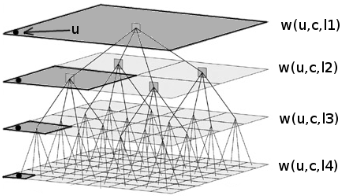
\includegraphics{obr1}
\caption{ Location-aware concept weighting based on quadtree
 regions}
\end{figure}

Our   user   model   is   defined   as   vectors   of   weighted 
concepts partitioned in PR-quadtree regions [5]. PR
-quadtree 
is a tree that has one root and every node of the s
tructure has 
0 or 4 children. It is used in geographic informati
on systems 
because of its advantages that were the reason why 
we chose 
this data structure over the others

\begin{itemize}
\item{every region have similar number of entities,}
\item{live partitioning,}
\item{conserve space,}
\item{parent region connection,}
\item{fast location to region lookup.}
\end{itemize}

Connection   between   child   and   its   parent   nodes   is 
important to fast location lookup, when  we want to 
add new 
entities (users) to a region map, or to be exact, i
n microblog 
domain,  when  the  user  tweeted  from  a  location.  We  d
o  not 
need to scan 
all
 the regions and then find those that matches, 
it  is  sufficient  to  traverse  a  tree  from  main  node 
to  its  child 
using  quadtree  structure,  this  operation  consumes  O
(
log
  n) 
time. 
We  can  see  an  example  of  a  visualisation  of  quadtre
e  in 
Figure  2  that  was  created  for  users  of  Twitter  with
  locality 
obtained  by  geotagging  locality  field  in  user  profi
le.  Those 
users  were  selected  according  to  their  high  tweet  c
ount.  It 
resembles  the  world  map  and  its  density  of  populati
on.  The 
parts of the map where many users are located (or a
ssociated 
with),  are  smaller  regions;  the  map  is  more  partiti
oned.  It 
means  for  the  user  model  that  users  living  in  more 
crowded 
quadtree  regions  have  user  model  that  is  based  on  s
maller 
surroundings. 
It  is  important  that  the  quadtree  is  actually  a  tre
e,  thus 
every  user  is  modeled  in  its  closest  surrounding  re
gion,  but 
also  in  parent  regions  ending  in  the  global  node.  T
hat 
supports  the  idea  that  the  user  is  affected  by  its 
surrounding 
with   various   dimensions.   For   example,   there   are   new
s 
relevant  only  for  one  city,  other  news  for  country 
and  some are  independent  on  region,  so  there  are  no  traces  t
hat  news 
are significant in a particular region more than in
 other. 
Our  location-aware  model  uses  at  most  M(log 
n
)  times 
more  data  than  the  traditional  model  (
n
  is  maximal  number 
of  regions).  It  means  that  all  the  processing  is  a 
bit  slower. 
When   considering   the  improvements   of   user   model   we 
believe it is a very good trade-off.

\section*{III.   EVALUATION: NEWS RECOMMENDATION}

The   location-aware   enhancements   we   propose   retain 
generality  of  the  user  model.  However,  since  it  was
  created 
while  focusing  on  recommendation  of  web  content  (us
er 
links  or  news  in  a  particular  locality  or  global  ne
ws),  we 
evaluated the model with respect to this purpose. W
e use the 
defined user model for recommendation, i.e., we dea
l with a 
ranking  problem,  how  to  provide  a  user  with  ordered
  list  of 
weighted  links  (to  web  content)  based  on  their  rele
vance  to 
the user (with respect to time and location).  
We   quantitatively   evaluated   our   user   model   on   the 
UMAP2011  Tweets  dataset
1
  acquired  by  Abel  et  al.  [2]  by 
performing   a   synthetic   evaluation.   The   dataset   cont
ains 
2 316 204 tweets posted by 1619 users. 
We   performed   the   evaluation   as   a   sequence   of   the 
following steps: 

\begin{itemize}
\item{User model acquisition}
\item{News recommendation}
\item{Results evaluation}
\end{itemize}

In the first step we acquired user model by preproc
essing 
tweets,   enriching   tweets   based   on   link   analysis   and
subsequent  location-aware  user  model  creation.  Then
  we 
simulated  recommendation  of  news  for  users  in  the  d
ataset 
and evaluated the results by applying traditional i
nformation 
retrieval measures. 
Due  to  size  of  social  networks  the  number  of  users 
and 
amount  of  content  they  produce  is  enormous.  Hence  t
he 
scalability of our algorithms had to be considered.
 We chose 
MapReduce    programming    model    as    a    platform    for evaluation.  We  used  Google  Hadoop
2
 implementation  and 
Hive  for  SQL-like  syntax.  In  evaluation  it  showed  t
o  be  a 
good  decision,  because  it  was  about  30  times  faster
  on 
provided cluster than single-threaded solution. \\

\textit{A.  User model acquisition}\\

\textit{Tweets preprocessing}.  In  this  step  we  obtained  entities 
and  topics,  links,  users  and  locations  from  tweets 
using 
custom  JSON  parser  and  semantic  service  OpenCalais
3
. 
UMAP2011  Tweets  dataset  contains  tweets  description
  we 
used.  We  used  web  service  OpenCalais  for  every  twee
t  and 
the   result   obtained   was   JSON-formatted   text   contain
ing 
semantic  information  about  tweets.  We  parsed  entiti
es  and 
topics from obtained texts.  
In  order  to  obtain  localities,  we  got  user  identifi
ers 
contained  in  dataset  and  then  we  questioned  Twitter
  API 
service  for  the  Twitter  user  profile.  We  parsed  tex
t  location 
from  JSON  output  and  we  used  batchgeo
4
 to  obtain  user 
locality.  
Tweets   enrichment
.   User   tweets   often   point   to   web 
content that contains information potentially relev
ant for user 
model [3]. There are 1 066 929 links in the dataset
 we used. 
We  obtained  the  text  of  those  links  and  its  topics 
and 
concepts  using  SemanticProxy
5
 service.  This  service  reads 
the  content  of  links  from  tweet  dataset,  it  filters
  header, 
footer,  navigation  and  other  irrelevant  content  fro
m  HTML 
and then it extracts the entities with probability 
and the topic 
of link. Those entities and topics were added to us
ers’ tweets 
as  an  enrichment  with  a  goal  to  improve  the  user  mo
del, 
because people are usually interested in content of
 links they 
tweeted, so it characterize them better. 
Then we downloaded entities and topics from the fet
ched 
content  using  OpenCalais  (Note  that  there  is  also  U
MAP 
2011  News  dataset,  a  dataset  of  news  crawled  from  R
SS  of 
nyti.com,  bbc.com  and  cnn.com:  there  are  77 860  new
s  that 
consist  of  1 896 328  entities.  However,  only  12k  en
tities 
were  linked  with  actual  tweets  using  exact  match,  h
ence 
making this dataset insufficient.) 
User  model  creation
.  We  assigned  users  a  location  they 
tweeted   from.   Users   tweeted   from   all   over   the   world
; 
however,  only  66 \%  of  them  were  successfully  geo-ta
gged 
by  batchgeo.  We  further  used  only  tweets  and  links 
from 
those  users  to  show  location  aspect  of  user  models.
  We 
assigned  users  with  location  to  regions  represented
  by  PR-
quadtree using PR-quadtree creation algorithm (see 
Location 
Modeling in section II). We decided to use at least
 100 users 
per region and then we filtered out those containin
g less than 
20,  because  too  small  regions  would  be  useless  (we 
would 
create  regions  based  on  too  few  users  and  regions  w
ould 
model  particular  users,  not  common  local  characteri
stics). 
We  chose  those  parameters  based  on  characteristics 
of  the 
UMAP2011  Tweets  dataset.  Finally  we  had  53  regions 
in 
PR-quadtree. When  the  model  is  being  created,  tweets  with  enrich
ed 
metadata are arranged to regions based on location 
and time 
period.  We  used  one  week  as  time  period.  After  weig
hting 
user models were created. \\
\textit{B.   News Recommendation}\\
We used a general synthetic evaluation approach use
d in 
machine  learning,  where  we  created  user  models  from
  train 
data  and  then  tested  (evaluated)  those  models  on  ot
her,  test 
examples. In our work, we used tweets from first ni
ne week 
periods of time for user model creation and the las
t one week 
period   for   recommendation.   The   same   approach   was 
employed  by  Geo  et  al.  in  [7],  whom  we  want  to  comp
are 
with. 
We recommended  top 
n
  links from  testing dataset  to  our 
combined  user  models.  Then  we  checked,  if  users  act
ually 
posted a link that matched one of the recommended l
inks. In 
related work authors typically use information abou
t web site 
accesses  (e.g.,  logs  of  visited  sites  obtained  from
  yahoo 
toolbar  [12]).  However,  in  the  UMAP2011  datasets  su
ch 
information  is  not  available.  In  fact,  Gao  et  al.  [
7]  used 
UMAP2011 News dataset that is much smaller than all
 links, 
which  we  consider.  They  also  linked  news  to  tweets 
by 
utilizing  similarity  measure  to  find  most  relevant 
links  for 
tweets  instead  of  exact  match  between  a  tweet  and  a
  link, 
i.e.,  placing  that  link  into  the  tweet.  In  our  appr
oach,  we 
know exactly what links are contained in tweets so 
we do not 
relate on less accurate information. 
To  generate  recommendations  we  used  cosine  similari
ty 
that  is  commonly  used  in  recommendation  systems.  De
spite 
its  simplicity  this  method  is  sufficient  since  our 
aim  is  to 
evaluate   and   compare   models   and   not   to   devise   most 
accurate   recommender.   In   order   to   compute   similarit
y 
(suitability)  of  a  web page 
N
j
 with  respect to the  user  model 
M
i
, we use the following equation: 
\begin{equation}
sim(M,N)={(c,relevancy(c,url))|c}
\index{id5}
\end{equation}
\\
where  model  of  web  document 
N
  is  represented  as  a  vector 
of concepts with relevancy retrieved from content o
f links by 
SemanticProxy.  
The recommendations were generated based on locatio
n-
aware  model,  for  every  region  the  user  belongs  to. 
The 
smaller  the  region  was,  the  more  the  user  model  was
  aware 
of  local  trends.  We  used  an  averaged  recommendation
  from 
all  recommendations  from  every  region  of  a  user.  As
  our 
approach is based on  location  modeling based on  com
posite 
regions  (each  region  has  its  quadtree  parent  node  r
egions), 
we  capture  local  trends,  but  we  are  also  aware  of  g
lobal 
trends.  
Since we obtained many recommendations for each use
r, 
we selected top-n to select only the  most relevant 
web news 
documents  for  the  user.  The  result  set  consisted  of
  triplets: 
user,  link  and  relevancy  for  each  of  962  users  (inv
olved  in 
both  training  and  testing).  The  number  of  recommend
ations 
for each user varied based on actual value of 
n
 parameter.  
To  evaluate  the  results,  we  used  standard  measures 
used 
for   recommendation   evaluation,   such   as   precision   at
   n 
(
P@n
),  recall  (
R
),  F-measure  (
F
1
)  and  Mean  Reciprocal 
Rank  (MRR),  which  show  various  aspects  of  quality  o
f  the 
model:

\begin{equation}
P=1\\
R=2\\
F=2\\
\index{id6}
\end{equation}
\\
where 
U
  is  set  of  all  users, 
RET
(
u
)  is  set  of  retrieved 
documents   for   user 
u
   and 
REL
(
u
)
is   set   of   relevant 
documents for user 
u
. For mean reciprocal rank we borrowed 
definition from [14]: 
\begin{equation}
MRR=1
\index{id7}
\end{equation}
\\
where 
Q 
is  a  query.  In  our  case,  a  query  constitutes  a  user
model  involved  in  recommendation.  In 
MRR
  we  weight 
quality  by  rank  (position)  of  first  relevant  docume
nt  in 
ordered recommendation list. 
It  is  important  to  note  that  our  evaluation  and  com
bined 
user   model   had   more   parameters   (see   Table   I).   When 
evaluating   news   recommendation   we   performed   several
simulations in order to determine influence of para
meters.  \\
\\
\\
\\Table 
\\

To compare the quality of model we create our propo
sed 
location-aware model and existing “global” model [7
]. 
We   used   entities   or   topics   as   concept   types   from 
OpenCalais for user and trend models [2].  
As  a  weighting  function  we  used  TF-IDF  and  t-TF-
IDF [7] We  also  experimented  with  different  influence  of  tr
ends 
on the combined model (parameter 
d
), which defines ratio of 
user  and  trend  model.  Due  to  the  finding  of  Gao  et 
al.  [7], 
user model in combined model is more important than
 trend 
model, so we focused the 
d 
parameter close to 1. 
In order to observe characteristics in relation to 
a number 
of recommendations there is a top-
n
 parameter.

\textit{C.    Results and discussion}\\
We    evaluated    local    and    global    combined    model 
performing  simulations  with  together  160  combinatio
ns  of 
the parameters by applying the described measures. 
First, we compared influence of the parameters on t
he F-
measure.   The   best   and   worst   values   of   F-measure   for
particular setup are depicted in Figure 3. The most
 important 
parameter    influencing    the    recommendation    was    trend 
influence 
d
  in  combined  user  model.  It  was  revealed  that 
model based on user’s interests was 8 times better 
in average 
than model when only trends are considered accordin
g to F-
measure.  Entity-based  models  were  twice  as  good  as 
topic-
based  models.  Number  of  recommendations 
n=5
  was  1.5 
times  better  then 
n=100
  in  average.  t-TF-IDF  improves  the 
model   as   much   as   4   \%   when   compared   with  TF-IDF. 
Location  awareness  of  models  improved  models  by  ave
rage 
by 2 \%.

The   presented   F-measure   values   were   averaged   for 
various  setups  to  give  a  basic  picture  of  results. 
Particular 
models  were  much  better, although  some  setups  were 
worse 
than others. We focused on location awareness of mo
del and 
analyzed those results in more detail.  
Tab.  II  shows  a  comparison  based  on  Precision,  Reca
ll, 
F-measure   and   Mean   Reciprocal   Rank.   Location-aware 
model improved in average Precision, Recall and F-m
easure 
increased  by  2  \%,  while  MRR  decreased  by  1.7  \%.  MRR
measures  the  position  of  first  relevant  result.  We 
suppose 
MRR was decreased because there were new relevant r
esults 
in  local  model  given  for  users  that  had  0  relevant 
results  in 
top-n recommendation list based on global model. In
 case of location-aware  models  there  were  new  results  with  l
ower 
position  that  decreased  MRR  measure.  As  F-measure  w
as 
improved, decreased  MRR  does  not  necessarily  mean  w
orse 
model.   MRR   using   all   recommendations   evaluated   on 
models  with  parameters  with  best  F-measure  showed  s
mall 
improvements. \\

We  found  that  the  best  model  according  to  Precision
, 
Recall  and  F-measure  is  entity-based  location-aware
  t-TF-
IDF  user  model (
d=1
). In  Figure 4a  we  can  see its behavior 
when 
n
  parameter  changes.  We  can  observe  a  standard 
Precision  and  Recall  “pattern”  where  Precision  is  d
ecreased 
and   Recall   increased   when 
n
   is   increased.   The   best 
recommendation  according  to  F-measure  was  obtained 
for 
n=10
. 
The  best  location-aware  improvement  of  the  model  wa
s 
achieved  for  combined  model  (
d=0.8
)  with  t-TF-IDF  as 
weighting function, topic concept type with 
n=10.
 It exceeds 
27 \%  of  improvement  when  considering  Precision  (see
  also 
Figure  4b).  Trend  models  were  improved  more  than  us
er 
based models. Location-aware models were equal or b
etter in 
67.5 \% than global models according to Precision, 7
7.5 \% by 
Recall, 67.5 \% by F-measure and 52.5 \% by MRR. 
We found that Mean Reciprocal Rank was the best whe
n 
d=0.4
   in   combined   model
.
   In   [7]   similar   results   were 
reported  so  we  confirm  these  findings  and  we  conclu
de  that 
combined  user  model  consisting  of  user  model  and  tr
end 
model improves MRR measure. 
The  best  model  yielded  4  \%  precision.  It  is  importa
nt  to 
note  that  there  was  a  huge  information  overload  in 
this 
dataset  and  we  were  recommending  content  to  every  u
ser 
from 962 users.  
It  is  important  to  discuss  limitations  of  evaluatio
n  we 
used.   It   could   possibly   result   in   even   better   resul
ts. 
Recommended  content  was  marked  as  relevant  only  whe
n 
there was exact match in URL. We recommended also o
ther 
relevant content that was evaluated as irrelevant b
ut in fact, it 
could  be  relevant  as  well.  Twitter  users  often  used
  URL 
shortener  services  (such  as  http://bit.ly/).  We  rec
ommended 
URLs    linked    to    relevant    content,    but    shortened    by 
shorteners. In our evaluation we did not link short
ened URLs 
from   more   shorteners   pointing   to   the   same   content. 
In 
addition,  there  was  more  content  that  was  not  exact
ly  the 
same,  but  it  was  similar,  e.g.,  story  about  some  co
mpany 
mentioned   in   bbc.com,   nyti.com   and   cnn.com.   In   our 
experiments  we  considered  that  this  content  was  not
  the 
same   (only   one   recommended   link   was   evaluated   as 
relevant).  That  means  that  the  Precision  and  other 
measures 
were actually better than evaluated. However, our e
valuation 
\\ table
\\

plan was consistent across all the models evaluated
, so it was 
appropriate for comparison of those models.\\
\textit{IV.   CONCLUSIONS}
\\
In  this  paper  we  proposed  a  location-aware  user  mod
el 
for  web  content  recommendation.  We  followed  the  wor
k  of 
Gao  et  al.  [7]  and  researched  how  location  aspects 
of  both 
users  and  trends  (represented  by  user  and  trend  mod
els, 
respectively)  relate  to  the  quality  of  combined  use
r  model 
and how it affects recommendation of web (news) con
tent. 
We performed an evaluation of the combined user mod
el 
with  various  parameters.  We  confirmed  our  hypothesi
s  that 
location-awareness  can  improve  the  quality  of  model
,  as 
much  as  27  \%  for  best  setup  and  2  \%  in  average.  The
  best 
user  models  created  when  considering  Precision,  Rec
all,  F-
measure  and  Mean  Reciprocal  Rank  were  location-awar
e 
models  using  t-TF-IDF  as  weighting  function,  i.e., 
those 
considering  temporal  characteristics  reflecting  tre
nds.  We 
also found that personalization based on user is 8 
times better  
than  one  based  on  trend  (in  terms  of  F-measure).  Ho
wever, 
mix of user and trend in combined model can improve
 Mean 
Reciprocal Rank. 
We  consider  the  results  we  obtained  very  reasonable
. 
They  show  that  location  aspect  in  user  modeling  is 
very 
important especially in large scale systems such as
 nowadays 
very  popular  microblogs.  We  believe  the  importance 
of 
location-aware  user  modeling  will  be  even  more  incr
eased 
with  the  huge  boom  of  smartphones  and  tablets  with 
even 
higher support for location data production and uti
lization. 


\end{document}